\documentclass{article}
\usepackage[utf8]{inputenc}
\usepackage{polski}
\usepackage{graphicx}
\usepackage[margin= 2.5cm]{geometry}
\usepackage{amsmath}
\usepackage{float}
\usepackage[section]{placeins}

\title{Wskaźnik MACD}
\author{Piotr Pesta}
\date{Marzec 2022}
\setlength{\parindent}{20pt}
\graphicspath{{./Graphs/}}

\begin{document}
\maketitle

\section{Wstęp}

    Celem projektu było zaimplementowanie wskaźnika MACD (Moving Average Convergence Divergence), który pozwala na podstawie analizy danych historycznych
    wyznaczać momenty kupna i sprzedaży udziałów. Wskaźnik ten składa się z dwóch krzywych: MACD oraz Signal.
    Implementacji dokonałem w języku Python z wykorzystaniem bibliotek pandas oraz matplotlib.
    Dane wejściowe to plik .csv o zawierający informacje o cenach udziałów z konkretnych dni. 
    Jako wartość udziałów w danym dniu przyjąłem cenę zamknięcia z tego dnia. Do algorytmu obracającego akcjami podajemy ok. 1000 rekordów.

\section{Analiza zadania}

    W celu określenia na podstawie wskaźnika MACD momentów kupna i sprzedaży akcji należy obliczyć
    dwie średnie kroczące z wartości udziałów:
    \begin{itemize}
        \item krótkookresową - 12 okresów
        \item długookresową - 26 okresów
    \end{itemize}

    \noindent Następnie wartość MACD uzyskujemy odejmując średnią długookresową od krótkookresowej.
    W celu obliczenia Signal należy obliczyć średnią krocząca z MACD z 9 okresów. 


    Do obliczenia średnich kroczących skorzystałem z poniższego wzoru:
 
        

    \begin{align*} 
        EMA_{N} &= \frac{p_{0} + (1-\alpha)p_{1} + (1-\alpha)^2p_{2} + \ldots + (1-\alpha)^Np_{N}}{1 + (1-\alpha)+(1-\alpha)^2 + \ldots + (1-\alpha)^N} \\
        \mathit{Gdzie:} & \\
        \alpha &= \frac{2}{N + 1} \\
        N &- liczba \; okres \mathit{ó} w \\
        p_{i} &- pr\mathit{ó}bka \; z \; i-tego \;dnia, \;p_{0}\; jest\; pr\mathit{ó}bk\mathit{ą} \;z \;aktualnego \;dnia, \;p_{N} \;to \;pr\mathit{ó}bka \;sprzed \;N \;dni.
    \end{align*}

    Punkty, w których krzywa MACD przecina Signal od dołu są sygnałem do kupna akcji oraz zapowiadają trend wzrostowy.
    Natomiast punkty, w których MACD przecina Signal od góry, są sygnałem sprzedaży akcji i zapowiedzią trendu spadkowego. 

\section{Analiza skuteczności i przykłady działania}
    \begin{figure}[!htb]
        \noindent\makebox[\textwidth]{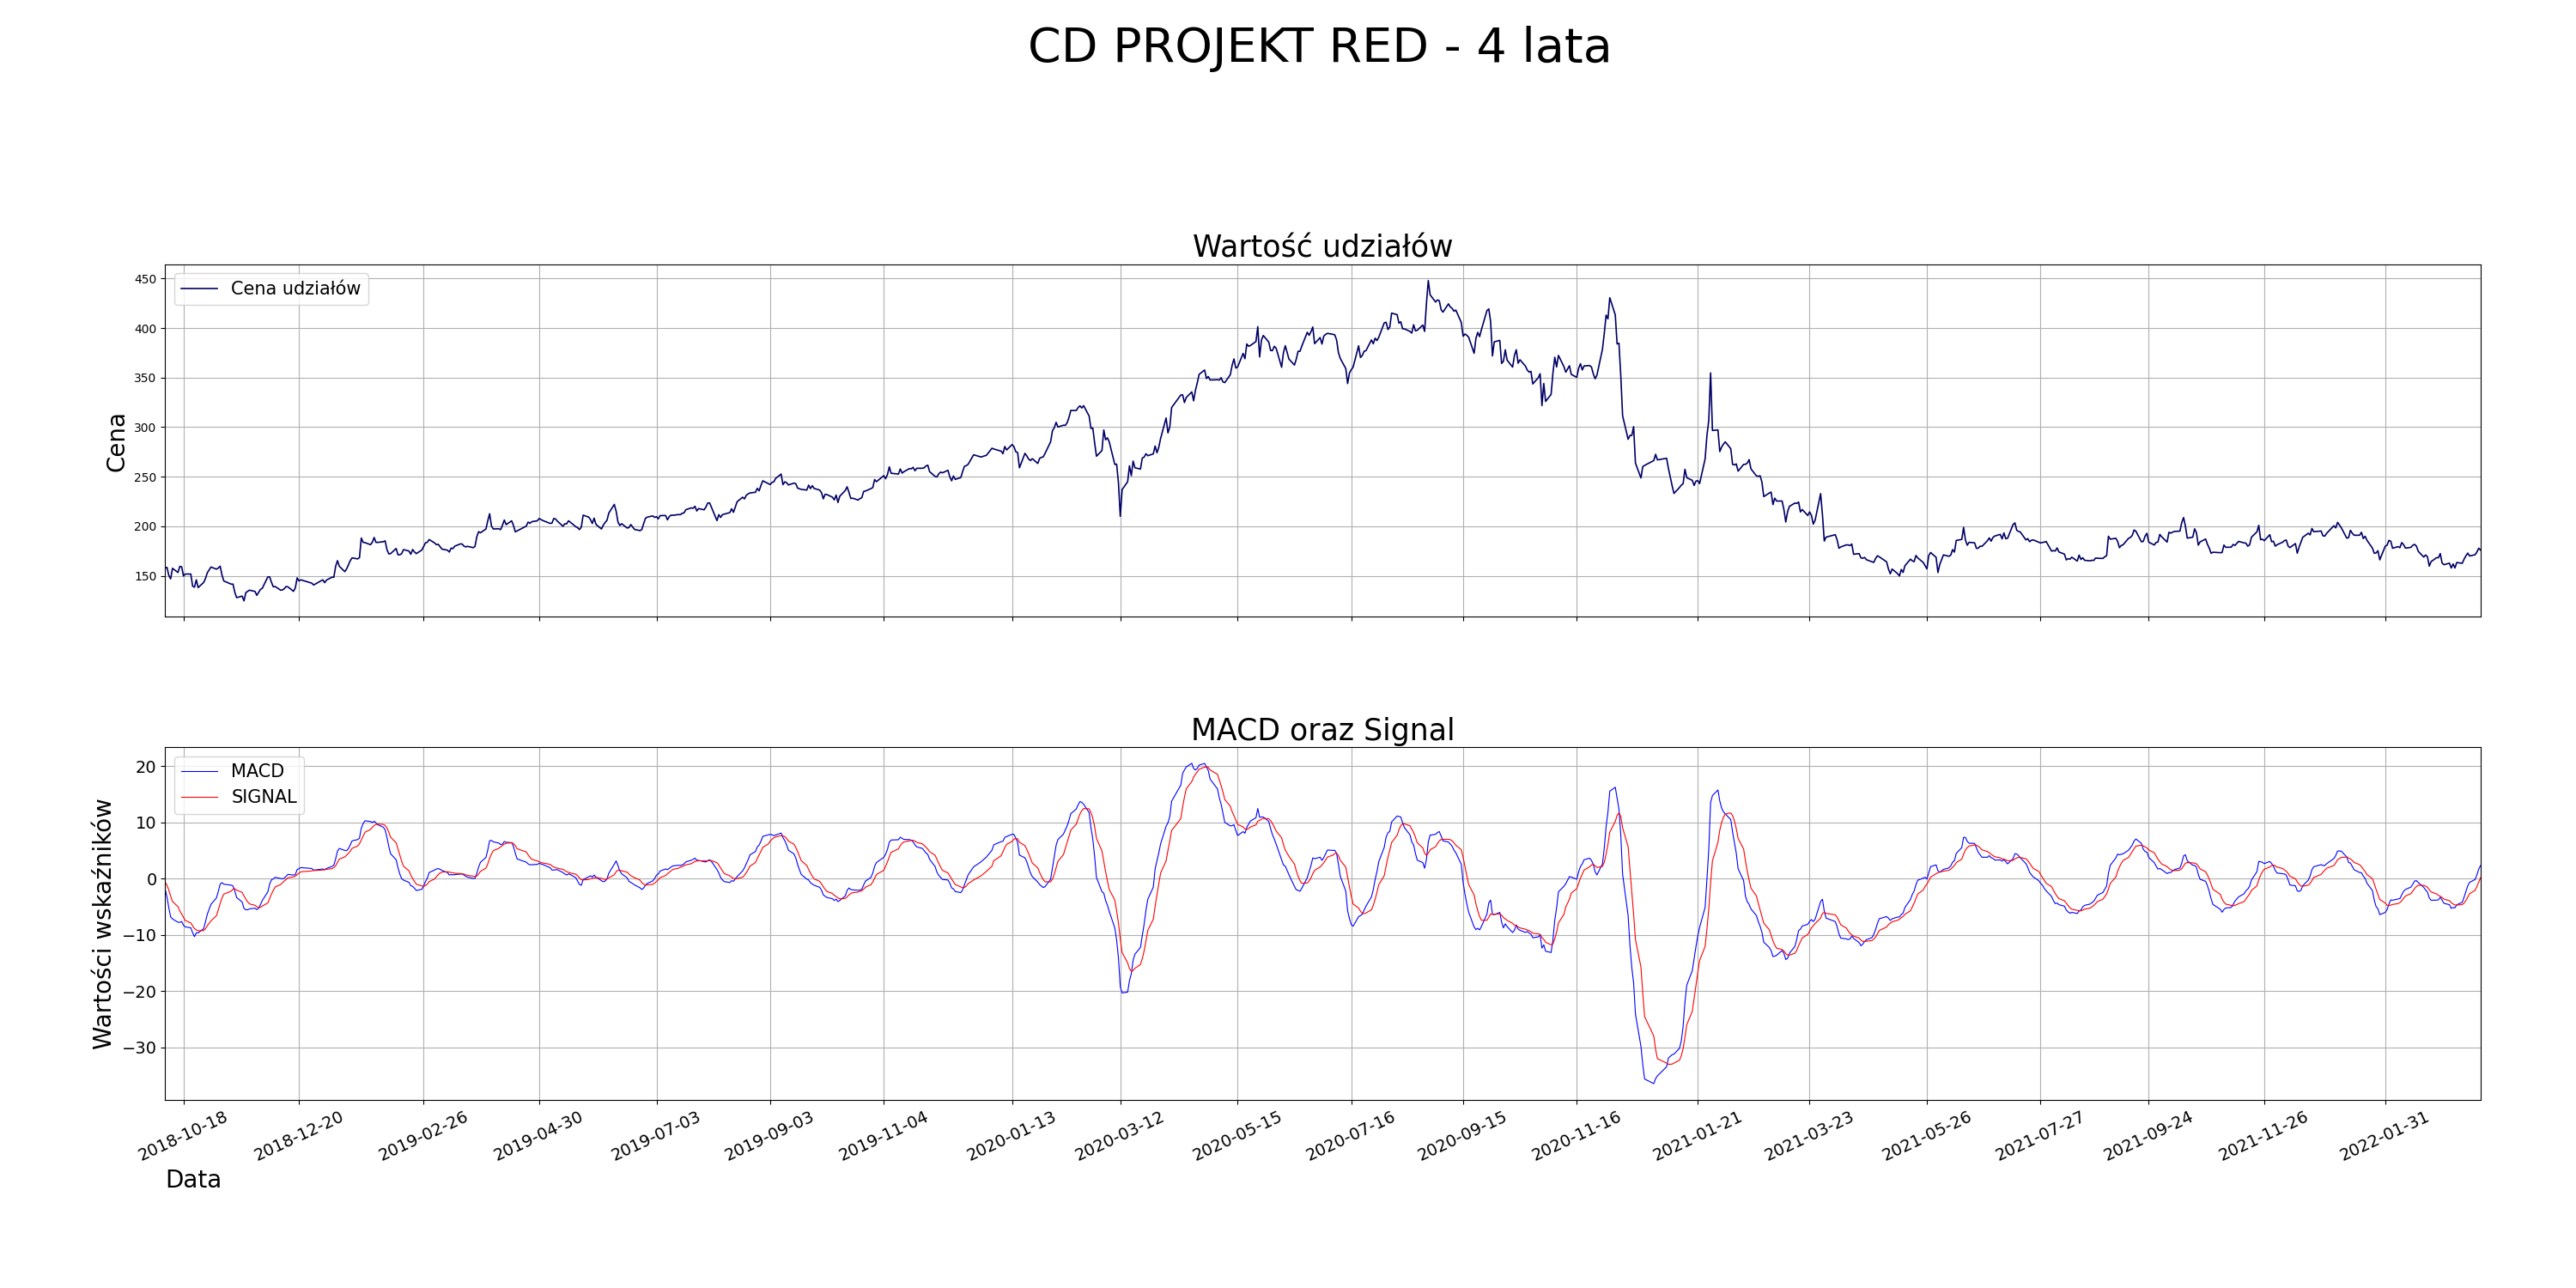
\includegraphics[width=\paperwidth]{CD PROJEKT RED - 4 lata.png}}
        \caption{Wykres ceny udziałów CDR oraz obliczonych na ich podstawie MACD oraz Signal. Wykres ten składa się z ok. 900 cen zamknięcia}
    \end{figure}

    

\section{Analiza przydatności MACD do inwestowania}

    Tutaj analiza algorytmu do inwestowania

\end{document}